\chapter{Program minimization}\label{chap:minimization}

As described in the first chapter, debugging is a time-consuming task.
Any amount of help with debugging is always appreciated by developers.
In this project, we attempt to help by providing means to minimize the 
debugged program w.r.t. a given runtime error.
The minimization's goal is to reduce the amount of source code programmers 
must go through when debugging, thus speeding up the process.
The size reduction of the program should be fully automated and reasonably 
fast on simple inputs.
Furthermore, it should correctly handle any source code from the program 
domain specified below.
Great attention is given to the accuracy with which the minimizing algorithms 
work and their time efficiency.

The domain in which the algorithms that are shown below operate can be 
described as small and simple projects.
The presented approaches take into consideration code written in C and C++.
Support for more complicated concepts of those languages, such as templates,
is omitted.
Additionally, programs that involve multiple threads and other advanced
features that might trigger non-deterministic behaviour are also not taken 
into consideration.
Programs that rely on randomly generated numbers during their runtime do not 
fit into the domain as well. 
This is because executions of multithreaded and random programs cannot be 
easily reproduced.
Instead, the program minimization described in this project focuses 
on simple single-threaded console applications with consistent executions.

The problem of program minimization while preserving runtime errors can be 
described as follows.
Assume that a developer has encountered a runtime error in his application.
Using logging or debugging tools, he can extract the stack trace at that 
given point.
The stack trace provides valuable information for a minimizing algorithm.
The presented algorithms notably require a description of the error and 
the source code location at which the error was produced.
Based on the described scenario, we can draw the following definitions.

\begin{defn}[Location]\label{def04:1}
  Let $loc$: $\mathcal{S} \mapsto \{x | x = (file, line, col)\}$, 
  where $\mathcal{S} = \{S_1, S_2, \ldots, S_n\}$ 
  is the set of program's statements.
  We call the result of $loc(S_i)$ the \emph{location} of statement $S_i$.
\end{defn}

The source code's location is specified by a file name, the line number, and 
on that line, the number of characters from the left.
The location could be described in further detail by including starting and 
ending points.
However, in this simplified description, only the starting point is taken 
into consideration.

\begin{defn}[Failure-inducing statement]\label{def04:2}
  Let $E = (location, desc)$ be a runtime error specified by its location 
  and description. Let the program $\mathcal{P} = (S_1, S_2, \ldots,\-S_n)$
  result in $E$ upon execution.
  We call $S_i$ the \emph{failure-inducing statement} of 
  $E$ if $loc(S_i) = E(location)$.
\end{defn}

Failure-inducing statements are the sites from which an error was thrown.
That means the statements were present at the error's location when the error 
occurred.

Having found the site's source code location, the developer can now 
investigate the source code for a potential bug.
In the process, he might consider the values of application arguments 
present at launch-time and change his debugging process accordingly.
Nonetheless, the developer has to look through the source code to find 
the error's root cause.
This exact point is where the source code size reduction starts being 
beneficial.
Using static and dynamic analysis, it is possible to effectively and 
safely remove unnecessary source code.
Such code includes statements, declarations, and expressions that do not 
affect the program's state at the point given by the error.
With additional verification, it is also possible to remove code constructs 
that affect the state, but the error occurs regardless of whether they 
are present or not.

The reduced program's source code can then be used for debugging the given
runtime error.
The newly generated program has to fulfill the following invariant.

\begin{invar}[Location alignment]\label{invar04:1}
  Every program $\mathcal{P'}$ created by reducing the original program 
  $\mathcal{P}$ based on dynamic information given by the execution of
  $\mathcal{P}$ with arguments $A$ must result in the same runtime error $E$.
  The error's absolute location can differ; it must, however, occur in the 
  same context.
\end{invar}

The rule specifies that a program must end in the same runtime error 
as the original program to be considered a correctly reduced variant.
Though, with the change to the program's size, the location 
of failure-inducing statements also changes.
In $\mathcal{P}$, the error's location in the file should be lower compared 
to $\mathcal{P'}$ since $\mathcal{P'}$ has less code in general.
Stress is placed on the location's context in which the error arises.
As long as locations in $\mathcal{P'}$ are adjusted based on those in 
$\mathcal{P}$, the absolute location of the error does not matter.

Figure~\ref{lst:reductionexample} contains an example of $\mathcal{P}$ and its 
minimal variant $\mathcal{P'}$. 
All statements that do not directly contribute to the specified 
runtime error are removed.
A non-minimal variant might contain additional non-impactful lines, 
such as line 37.

\begin{figure}[p]
\begin{minipage}{0.46\textwidth}
\begin{lstlisting}[basicstyle=\small, caption=Program $\mathcal{P}$.,
  language=C++, label={lst:reductionoriginal}]
#include <stdio.h>
#include <stdlib.h>

long get_factorial(int n)
{
	// Missing the stopping 
	// constraint 
	// => segmentation fault.
	return (n * 
		get_factorial(n - 1));
}

int main()
{
	const int n = 20;
	long loop_result = 1;
	
	for (int i = 1; i <= n; 
		i++)
	{
		loop_result *= i;
	}
	
	long recursive_result = 
		get_factorial(n);
	
	if (loop_result != 
		recursive_result)
	{
		printf("%ld, %ld\n", 
			loop_result, 
			recursive_result);
			
		return (1);
	}
	
	printf("Success.\n");
	
	return (0);
}
\end{lstlisting}
\end{minipage}
\hfill
\begin{minipage}{.45\textwidth}
\begin{lstlisting}[basicstyle=\small, caption=Minimal va\-riant $\mathcal{P'}$., 
  language=C++, numbers=right,
  label={lst:reductionminimal}]
#include <stdio.h>
#include <stdlib.h>

long get_factorial(int n)
{
	// Missing the stopping 
	// constraint 
	// => segmentation fault.
	return (n * 
		get_factorial(n - 1));
}

int main()
{
	const int n = 20;
	
	
	
	
	
	
	
	
	long recursive_result = 
		get_factorial(n);
	
	
	
	
	
	
	
	
	
	
	
	
	
	
}
\end{lstlisting}
\end{minipage}
\caption{A program resulting in a segmentation fault error and its 
minimal erroneous variant. 
The variant is stripped off all statements unnecessary for the error 
to occur. }
\label{lst:reductionexample}
\end{figure}

So far, this chapter has talked about both minimization and reduction 
simultaneously. 
It is crucial to make a distinction between those two terms. 
In this context, the reduction is simply the process of making the program 
smaller in size. 
The reduced program must also result in the same runtime error. 
Minimization is built on the same rules as reduction; however, it must 
fulfill one additional property. 
No statement of the minimized program can be removed while preserving 
the error. 
The task of reduction is more straightforward than that of minimization. 
Finding the program's minimal variant is computationally infeasible for 
large inputs. 
Whereas reducing the program to a rough approximation of the optimal 
solution can be done in polynomial time. 
Although this project focuses on minimal program variants, we recognize that 
it is expensive to compute them. 
Instead, we use reduction and minimization interchangeably throughout 
the text.

Minimization of programs requires two steps—first, the removal of chunks 
of the given source code. 
The following sections describe several techniques of code removal. 
The naive approach is explained briefly. 
Possible improvements to that approach concerning runtime are then described. 
Subsequent approaches employ techniques discussed in 
chapter~\ref{chap:automated}. 
The method based on Delta debugging offers a modified version of 
the debugging algorithm. 
Another approach combines different types of slicing to achieve the best 
results.

Second, the minimization needs to perform a validation to determine whether 
the result meets the required criteria, i.e., minimality (or an approximation) 
and correctness.
The description of naive validation is shown in the sections below.

\section{Naive reduction}\label{chap:naive}

The simplest approach examined in this project is the naive removal of each 
source code statement.
This technique aims to try every possible variation of the code and find 
the smallest correct solution through trial and error.
All possible variations, both valid and invalid at compile-time, can be 
generated by separating the source code into units of statements, 
declarations, and expressions and removing one code unit at a time.

\begin{defn}[Code unit]\label{def04:3}
  Let $\mathcal{P}$ be a program consisting of a sequence of statements, 
  expressions, and declarations $(S_1, S_2, \ldots, S_n)$. 
  We call $U_i = (S_{i_1},\-S_{i_2},\-\ldots,\-S_{i_n}), 
  U_i \subseteq \mathcal{P}$ a \emph{code unit} if the sequence 
  $(S_{i_1}, S_{i_2}, \ldots, S_{i_n})$ is syntactically
  correct.
\end{defn}

A code unit represents any syntactically correct subset of the original 
program. 
Working with all code units is not practical in our case. 
Instead, we will focus on atomic code units. 
Atomic code units are the minor code units in the given program. 
For example, the atomic code unit might be a \icode{for} loop with its body 
or an assignment expression, such as \icode{x = 3;}.
The rest of the text will refer to atomic code units simply as code units. 

Algorithm in figure~\ref{alg:naive} describes the naive process. 
Once the input source code is provided, it is split into $n$ code units.
Every unit has two possible states: it is either kept or removed.
Let us represent each statement with a single bit. 
For a program $\mathcal{P} = \{S_1, \ldots, S_n\}$, we would suffice with 
a bitfield of size $n$. 
This bitfield would keep track of whether each bit is kept or removed. 
Statement $S_i$ is kept if the $i^{th}$ bit in the bitfield is set to $1$. 
On the other hand, $S_i$ is removed when the $i^{th}$ bit is set to $0$.
The bitfield representation is used for generating every subset of $n$ given
elements. 
It works by considering the bitfield as an unsigned binary number and 
gradually incrementing that number. 
With each increment, a new variant of the bitfield is generated. 
The very same approach can be used in naive minimization.
Analogically to generating every subset of a set of elements, this
variant generating algoritm results in $2^n$ possible variants.

\begin{figure}[h]
	\hrule height.8pt depth0pt \kern2pt
	\textbf{Input:} \\
	\hspace*{\algorithmicindent} $L \ldots$ location of the error. \\
	\hspace*{\algorithmicindent} $P \ldots$ the input source code. \\
	\hspace*{\algorithmicindent} $A \ldots$ the input program's arguments. \\
	\textbf{Output:} The reduced source code. 
	\hrule height.8pt depth0pt \kern2pt
	\begin{algorithmic}[1]
		\State $allVariants \leftarrow \{\}$
		\State $(C_1, C_2, \ldots, C_n) \leftarrow$ SplitIntoCodeUnits($currentVariant$)
		\State $bitField \leftarrow [{bit}_{n-1}, {bit}_{n-2}, \ldots, {bit}_0]$,  
			$\forall i \in 0 \ldots n-1 : bit_i = 0$
		\While{$\exists i \in 0 \ldots n-1 : bit_i = 0$}
			\State $bitField \leftarrow Increment(bitField)$
			\State $currentVariant \leftarrow (C_1, C_2, \ldots, C_n)$
			\For{$i \in 0 \ldots n-1$}
				\If{bitField[i] = 0}
					\State $currentVariant \leftarrow currentVariant \setminus \{C_{i+1}\}$
				\EndIf
			\EndFor
			\State $allVariants.Add(currentVariant)$
		\EndWhile
		\State $allVariants \leftarrow$ SortBySize($allVariants$, $Ascending$)
		\ForAll{$V \in allVariants$}
			\If{IsValid($V$, $L$, $A$)}
				\Return $V$.
			\EndIf
		\EndFor
		\State \Return none.
	\end{algorithmic} 
	\hrule height.8pt depth0pt \kern2pt
	\caption{Naive Statement Removal.} 
	\label{alg:naive}
\end{figure}

The naive time complexity is, therefore, the abysmal $\mathcal{O}(2^n)$.
Moreover, the $2^n$ variants require some verification and classification 
to determine whether they are minimal or not.
Nevertheless, we can be sure that a set of those $2^n$ variants contains 
the desired minimal variant.
The correctness of many of the invalid variants can be ruled out immediately
since they indeed are not syntactically correct.
The rest, however, must be adequately tested for the desired runtime error.

\subsection{Heuristics}

The algorithm can be sped up by using various heuristics. 
The search space normally contains variants that are syntactically or 
semantically incorrect. 
Generating such variants and validating them needlessly wastes time. 
We can overcome this issue by introducing a mechanism that validates some 
aspects of the variant beforehand. 
An example of such a mechanism is keeping track of code unit dependencies. 
Let us create a directed graph of dependencies. 
Each node of the graph represents a code unit in the input source code. 
There is an edge from node $u$ to node $v$ if the code unit $v$ is 
the subset of code unit $u$. 
It is natural to wonder what exactly do these edges achieve. 

\begin{figure}[H]
\begin{minipage}{0.46\textwidth}
\begin{lstlisting}[basicstyle=\small, caption=An if - else statement.,
  language=C++, label={lst:dependencycodeoriginal}]
if (x % 2 == 0)
{
	CreateEvenSpacedTable();
}
else
{
	CreateOddSpacedTable();
	trim = true;
}
\end{lstlisting}
\end{minipage}
\hfill
\begin{minipage}{.45\textwidth}
\begin{lstlisting}[basicstyle=\small, caption=An invalid variant 
of~\ref{lst:dependencycodeoriginal}., language=C++, numbers=right,
  escapechar=\%, label={lst:dependencycoderemoved}]
	
	
CreateEvenSpacedTable();
	
	
	
CreateOddSpacedTable();
trim = true;
%%

\end{lstlisting}
\end{minipage}
\caption{An example of a semantically incorrect variant. The original source
code snippet in Listing~\ref{lst:dependencycodeoriginal} performs different 
actions in each branch. A variant with removed control statements shown in
Listing~\ref{lst:dependencycoderemoved} performs both of those inconsistent 
actions during the same run.}
\label{lst:dependencycode}
\end{figure}

Figure~\ref{lst:dependencycode} attempts to illustrate the usefulness 
of those edges. 
The example shows an \icode{if - else} statement. 
Let us assume that the naive algorithm attempts to remove two code units. 
First, the code unit \icode{if(...)} is removed while keeping the statements 
inside the body. 
Second, the code unit \icode{else(...)} is removed while, again, keeping 
the statements inside the body. 
Originally, the input program would never run statements in those two 
branches in the same execution path. 
However, the generated variant invalidates the original behavior. 
The statements from those two branches will be run together. 
Such variant results in an obvious semantical error. 
While the described process might lead to a smaller failure-inducing program, 
we believe that such a program is incorrect. 

This semantical error can be avoided by validating the dependency graph 
mentioned earlier.
For this example, we start by creating a node $u$ for the \icode{if(...)\{\}} 
statement. 
Once we encounter the body of the \icode{if(...)} statement, we add it to 
the dependency graph as node $v$. 
The \icode{if(...)} statement's children also syntactically contain 
the \icode{else(...)\{\}} statement. 
Therefore, we add nodes $x$ and $y$ for the \icode{else(...)} statement and 
its body, respectively. 
The nodes $v$, $x$, and $y$ are subsets of $u$.  
This holds since the code unit $u$ contains both the \icode{if(...)} 
statement and other parts. 
Those parts include the statement's body, the else branch, and the body of 
the else branch. 
By completing the edges between the four nodes, we get the dependency graph 
that solves our issue. 

\begin{figure}[h]\centering
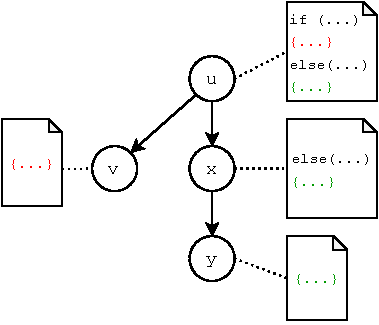
\includegraphics[scale=1.5]{dependency_graph}
\caption{A dependency graph of the source code shown in 
Listing~\ref{lst:dependencycodeoriginal}}
\label{img:dependencygraph}
\end{figure}

The graph, visualized on Figure~\ref{img:dependencygraph}, states that 
the body of the \icode{if(...)} statement depends on the \icode{if(...)} 
statement. 
Analogically, the \icode{else(...)\{\}} statement and its body depend on 
the \icode{if(...)} statement. 
We can use this information and only remove parent nodes if all their 
children are removed as well. 
This simple rule prevents invalid execution flow in the shown example. 
A variant generated by following this rule has the bodies of \icode{if(...)} 
and \icode{else(...)} only if \icode{if(...)} and \icode{else(...)} are 
present as well. 
Creating and following a graph of dependencies is a heuristic worth 
deploying in this project. 
It can also be extended further to include syntax errors. 
One such error that immediately comes to mind is referencing a removed 
declaration. 
Assume that the algorithm has generated a variant in which a variable 
declaration is removed, such as the one shown in Figure~\ref{lst:declref}.
The algorithm has not, however, removed usages of the declared variable. 
Such variant will fail at compile time. 
However, we can avoid generating this variant by creating edges from 
the variable declaration $u$ to variable references
$\{v_1, v_2, \ldots, v_k\}$. 

\begin{figure}[H]
\begin{minipage}{0.46\textwidth}
\begin{lstlisting}[basicstyle=\small, caption=A variable declaration and its 
usage.,
  language=C++, label={lst:declreforiginal}]
int factor = 3;
int x = 0xffff;

while (x > 0)
{
	std::cout << factor * x << "\n";
}
\end{lstlisting}
\end{minipage}
\hfill
\begin{minipage}{.45\textwidth}
\begin{lstlisting}[basicstyle=\small, caption=Reference to an invalid 
declaration., language=C++, numbers=right, label={lst:declrefremoved}]
int factor = 3;


while (x > 0)
{
	std::cout << factor * x << "\n";
}
\end{lstlisting}
\end{minipage}
\caption{An example of a syntactically incorrect variant. The declaration
of \icode{x} in Listing~\ref{lst:declreforiginal} was removed
in Listing~\ref{lst:declrefremoved}, while the usage of \icode{x}
was kept.}
\label{lst:declref}
\end{figure}

Another helpful heuristic involves predicting a variant's size before 
the variant is generated. 
We can significantly improve the best case and the average time complexities 
by introducing a size metric. 
Let us keep track of every code unit's size. 
Upon creating a bitfield, we can determine the variant's size by analyzing 
the bitfield. 
By summing up the size of each present code unit, i.e., each bit set to 1, 
we get the variant's total size. 
Such metrics can be used to enumerate bitfields and sort them based on their 
size. 
Once we have a sorted list of bitfields, we can start generating variants 
and validating them. 
We can then terminate the algorithm upon finding the first valid variant. 
This heuristic saves time and memory that would otherwise be spent on 
generating all possible variants.

\section{Delta debugging}\label{chap:deltaimplementation}

Zeller's Delta debugging \cite{Zeller99, Zeller02, Zeller01} has been 
described in detail in section~\ref{chap:delta}.
It is an automated debugging technique that focuses on input size reduction.
For a given input, Delta debugging attempts to find the input's 
smallest failure-inducing subset and isolate the a failure-inducing element 
using two algorithms.
This project is only concerned with the minimizing algorithm described in
section~\ref{chap:delta} and in the figure~\ref{alg:dd}.

For the rest of this section, the input will be referred to as 
a \emph{test case}.
Other than the test case, Delta debugging also requires the debugged program 
(in its executable form) and a method of validating its output.
Let us draw parallels between the mentioned requirements and this project's 
minimization task.
The input for program minimization is the given program's source code.
The code can be labeled as the test case Delta debugging takes.
It is essential to clarify that this Delta debugging usage does not utilize 
the source code as the debugged program.
Instead, it considers it as a given test case.
Then, we must specify the expected output and a method to validate it.
It is required that the program terminates with a given runtime error.
Let us label that runtime error and its location as the expected output.
Whenever the executed test case results in that particular error, we 
interpret the run as a failing one.
Every other terminating run will be interpreted as a passing one.
Lastly, we must define the debugged program.
In our case, to get from the test case (source code) to the expected 
output (a specific runtime error), the code must first be compiled 
and then executed.
The fitting debugged program is, therefore, a pipeline of a compiler and 
an execution environment.

The minimizing algorithm uses binary search in a greedy manner.
We have modified the way binary search is performed to better fit the input's
structure.
The original minimizing algorithm operates with partitions of equal size.
That is not necessarily the best approach for structured test cases such
as source code.
To give a concrete example, we can look at splitting a function definition
into two partitions.
Originally, we would get two syntactically invalid code snippets.
One would contain the function's head and the first half of its body.
The body would not contain the terminating curly bracket.
Similarly, the second would be missing an opening curly bracket.
Instead, it makes more sense to operate on code units.
A more detailed description of code units can be found in 
section~\ref{chap:naive}.

Initially, the test case is split into $k$ code units.
Those code units are then assigned into $n$ partitions of roughly the same 
size.
The number of partitions changes based on the current iteration, as described
in figure~\ref{alg:dd}.
In our case, each iteration compiles current test case subsets and executes 
them.
Executions are validated as described earlier and the algorithm reduces
the size of the test case gradually.
The result is roughly what we need - a minimal program variant approximation 
that fails with a particular error.
As was already mentioned in this chapter's introduction, the location of 
the error might differ based on the variant's structure.
Nonetheless, the location could be aligned based on the source code in 
an additional step, so that Invariant~\ref{invar04:1} holds.

The running time complexity of this modified algorithm, which is measured 
for the number of executed validations $v$, remains unchanged. 
Let us assume the test case consists of $k$ code units. 
Zeller and Hildebrandt\citep*{Zeller02} presented both the worst 
and the best case complexity as follows.

\paragraph{Worst case.} Two possible scenarios lead to the worst time 
complexity. 
First, every executed validation is inconclusive. 
That would lead to $v = 2 + 4 + 8 + \ldots + 2 * k = 4 * k$ validations. 
Second, the validation succeeds, i.e., finds a failing subset, for every 
last complement. 
This case given us $v = (k - 1) + (k - 2) + \ldots + 2 = k^2 - k$ validations.
Combined, these two scenarios lead to $k^2 + 3 * k$ validations at worst.

\paragraph{Best case.} The best case is the ideal scenario for utilizing 
binary search. 
We would be searching for a single failure-inducing code unit. 
This scenario leads to $2 * \log{}k$ validations.

Extracting an approximation of the minimal program variant after 
$\mathcal{O}(k^2)$ validations is undoubtedly practical. 
Especially when compared to the exponential time complexity of the naive 
approach described in section~\ref{chap:naive}. 
Those who desire the minimal variant might want to get the approximation 
first and provide it to the naive reduction. 
Nevertheless, there is no way of avoiding the exponential complexity when 
searching for optimal results.

\section{Slicing-based solution}\label{chap:systematic}

The slicing-based approach attempts to help with the shortcomings of 
the naive reduction described in Section~\ref{chap:naive}.
The algorithm described below combines static and dynamic slicing, 
minimization using Delta debugging, and the naive algorithm. 
The primary point is its preprocessing steps described below. 

It is crucial to keep the input size as low as possible due to the naive 
algorithm's exponential complexity.  
The input's size can be significantly reduced by slicing the input program 
as a preprocessing step.  
Let us compare the two slicing techniques described 
in Section~\ref{chap:staticslicing} and Section~\ref{chap:dynamicslicing} and 
apply them to our problem. 
The main focus of the comparison should be on two aspects - the size of 
the slice and the running time of the slicing algorithm. 

It is known that dynamic slices are the smallest they can be. 
However, they require information available at execution time. 
The question is whether running the program is necessary. 
We know that the program that is being minimized has been run before. 
Hence the availability of the information about the encountered runtime 
error. 
If the program ran deterministically, it would have to terminate in future 
executions as well.  
That is considering it would run with the same arguments as previously.  
We can therefore conclude that the program terminates.  
The time of the termination might vary depending on the purpose of 
the program.  
For server-like applications, it might take months to encounter an error 
at runtime. 
Static slicing does not suffer from the mentioned issue.  
It is inexpensive in terms of execution time regardless of the purpose of 
the sliced program. 

We see that static slicing is a significantly less expensive operation in 
terms of running time. 
Out of the two main issues concerning the previously discussed 
approaches - the input size and its execution time - static slicing helps to 
eliminate both. 
Both the input size and subsequent execution time could both be brought down 
further by using dynamic slicing.  
The usage of dynamic slices, as opposed to static, has the mentioned benefit 
of generating smaller slices.
On the other hand, it has definitive limitations. 
One such constraint is the requirement to run the said program. 

However, one can perform preprocessing steps to help dynamic slicing run more 
efficiently.  
Let us consider a program that performs multiple demanding tasks such as 
computations.  
These tasks are primarily independent, and their running time is longspun.  
Using dynamic slicing alone would be inconvenient.  
However, by first employing static slicing to remove these long-running 
unnecessary tasks, the program's execution time can be significantly reduced.  
The reduced program could then be sliced dynamically.  
The result would be a minimal slice at a fraction of the original time 
compared to dynamic slicing alone. 
This crafted ideal use case only concerns a very narrow range of existing 
programs.  
However, static slicing could be used before just any attempt at dynamic 
slicing due to its low running time. 

The improvement in the form of a static slice is genuinely convenient.  
However, checking whether the improvement has any effect before running 
dynamic slicing is not an easy task.  
The issue stems from the halting problem~\citep{Turing36} and 
Rice's theorem~\citep{Rice53}.  
The halting problem states that it is undecidable whether a program 
terminates on its particular input.  
Rice expanded the thought further by stating that all interesting semantic 
properties of a program are undecidable. 
Without proper and accurate means to determine many wanted properties, we 
are required to approximate them. 

Amongst such properties is the factor of how effective static slicing is.  
The approximation will be required in the following sections as well.  
In particular, the Section concerning program validation will look at this 
issue in more detail.  
One way of guessing the effectiveness of static slicing in terms of size 
reduction is by analyzing the program's branching factor. 
We can approximate static slicing's relative performance by employing 
a metric for the number and density of control-flow altering statements.  
It is assumed that programs with a high branching factor, i.e., with more 
control-flow-altering statements, are less likely to reduce their size 
during static slicing.
Nonetheless, slicing statically before doing so dynamically has been a rule 
of thumb for this project.  

We can, however, reap the benefits of both static and dynamic slicing while 
avoiding running the program. 
We need to follow the ensuing thought process. 
Since static slicing does not handle branching and other control statements 
nearly as efficiently as dynamic slicing, we can employ a trick to help.  
Using the same additional input information as dynamic slicing, i.e., 
program's arguments, we can provide more specific information to the static 
slicing algorithm.  
All that is required is to define the arguments with their respective values 
inside the code. 

This process will be referred to as \emph{argument injection}. 
Slices generated from this modified source code will be more precise since 
they will not contain unnecessary branching.  
It is important to restate that this modification only affects control 
statements dependent on the program's arguments.  
If the arguments do not appear in the original, unmodified static slice, 
their values will not affect the slice's size.  
Input modified using argument injection is guaranteed to be smaller or equal 
in size.

\begin{figure}[h]
	\hrule height.8pt depth0pt \kern2pt
	\textbf{Input:} \\
	\hspace*{\algorithmicindent} $L \ldots$ location of the error. \\
	\hspace*{\algorithmicindent} $P \ldots$ the input source code. \\
	\hspace*{\algorithmicindent} $A \ldots$ the input program's arguments. \\
	\textbf{Output:} The reduced source code. 
	\hrule height.8pt depth0pt \kern2pt
	\begin{algorithmic}[1]
		\State $S \leftarrow$ GetStatementAtLocation($L$)
		\State $variableList \leftarrow \{\}$
		\ForAll{$Expr \in S$}
			\If{$Expr$ is Variable}
				\State $variableList.Add(Expr)$
			\EndIf
		\EndFor
		\State $sliceList \leftarrow \{\}$
		\ForAll{$V \in variableList$}
			\State $sliceList.Add$(StaticSlice($P$, $L$, $V$))
		\EndFor
		\State $unifiedSlice \leftarrow$ Unify($sliceList$)
		\State $P' \leftarrow$ Compile($unifiedSlice$)
		\State $L' \leftarrow$ AdjustLocation($P$, $P'$, $L$)
		\State $sliceList \leftarrow \{\}$
		\ForAll{$V \in variableList$}
			\State $sliceList.Add$(DynamicSlice($P'$, $L'$, $V$, $A$))
		\EndFor
		\State $unifiedSlice \leftarrow$ Unify($sliceList$)
		\State $P' \leftarrow$ Compile($unifiedSlice$)
		\State $L' \leftarrow$ AdjustLocation($P$, $P'$, $L$)
		\State $P' \leftarrow$ PreciseReduction($P'$, $L'$, $A$)
		\State \Return $P'$.
	\end{algorithmic} 
	\hrule height.8pt depth0pt \kern2pt
	\caption{Minimization Based on Slicing.} 
	\label{alg:slicing}
\end{figure}

The proposed slicing-based solution is described in figure~\ref{alg:slicing}.
The input program is sliced statically w.r.t.
every variable available at the failure-inducing line.
The slices are then unified and given as the input to a dynamic slicer.
Similarly, the dynamic slicer generates slices w.r.t.
those potentially failure-inducing variables.
Those dynamic slices are then unified.

The intermediate result extracted after performing the two slicing types 
should be significantly smaller than the original program.
Since the result so far contains slices for multiple variables, it might not 
be minimal yet.
However, it can be assumed that it is valid, i.e., ends with the desired 
runtime error.
Using the observations made in Section~\ref{chap:naive} and 
Section~\ref{chap:deltaimplementation}, we can create an efficient and 
precise minimizing algorithm that takes care of the penultimate step 
in Figure~\ref{alg:slicing}. 
We utilize a pipeline of the minimizing Delta debugging algorithm and 
the naive reduction:
\begin{enumerate}
  \item The sliced intermediate result is fed to the Delta debugging 
  algorithm. 
  Due to its smaller size, the intermediate result contributes to a lower 
  amount of Delta iterations. 
  Therefore, Delta produces a local minimum more efficiently.
  \item The local minimum is optimized to the minimal variant by running 
  the naive reduction.
\end{enumerate}
Each step of the preprocessing and the pipeline leads to a smaller result. 
Additionally, each step benefits from the size reduction caused by 
the previous steps.

Another thought-about approach is hybrid slicing~\citep{Gupta97}.
This slicing technique is a compromise between static and dynamic slicing. 
The main benefit is that it produces smaller slices than static slicing. 
It also uses fewer resources than dynamic slicing. 
Hybrid slicing works by stopping at a set of breakpoints and using 
the information available at those points.
The comparison of hybrid slicing and the combination of static and dynamic 
could yield exciting results.
It can be assumed that hybrid slicing would be more effective on smaller 
programs with a short execution time.
The static-dynamic combination could work better on larger-scale 
applications, where static slicing can remove unnecessarily long-running 
chunks of code.

\section{Program validation}\label{chap:verification}

Once we generate a variant, we must ensure that the variant is correct. 
A correct variant results in the same runtime error as the original program. 
Moreover, the error must arise in the exact location. 
Section~\ref{chap:systematic} introduced the reader to Rice's theorem. 
This theorem is relevant in this chapter as well. 
By validating a variant, we are searching for a non-trivial property that 
cannot be obtained statically. 
This fact leaves two possible options. 
We can either determine the validness naively or approximate it. 
The latter is undoubtedly more exciting than the former. 
There is room for improvement when it comes to approximations. 
We could have come up with new methods altogether. 
While there might be several sophisticated validation techniques involving 
flow analysis, instrumentation, and even pattern recognition, we settled for 
a naive approach. 
This decision significantly lowers the amount of time required for this 
project. 
Furthermore, it allows us to focus on the minimization itself.

A simple way of finding the minimal failure-inducing subset of the program is 
by performing the following steps:
\begin{itemize}
  \item We attempt to compile each variant. 
  If a variant fails, we can rule it out definitely.
  \item We execute a static analyzer and check its warnings. 
  If a fatal warning or an error are generated, we rule the variant out as 
  well.
  \item We launch an execution environment that provides us with symbol 
  information of the running program. 
  We run the variant inside that environment and observe its output. 
  If the program crashes and generates the same error, it is considered 
  a valid variant. 
  Otherwise, it is ruled out.
\end{itemize}
These three steps define three barriers a program must overcome. 
Each barrier has a great chance of invaliding a typical variant. 
This chance increases the further into the verification the variant gets. 
Let us discuss these three steps in more detail.

\paragraph{Compilation.} The original program was compiled and executed by 
the user. 
We can expect a smaller variant to be compiled using the same compiler 
invocation as the original program. 
A successful compilation is the first step towards a valid reduced program. 
The compilation will rule out most syntactical errors. 
It does not, however, catch semantically invalid variants. 
Programs containing infinite loops and wrong control flow might pass 
the compilation just fine.

\paragraph{Static analysis.} The compilation above has its pitfalls. 
Invalid programs might be compiled without any issues. 
These programs would then cause issues when executing them: memory leaks, 
infinite loops, and pointless execution flow. 
By utilizing static analyzers, we increase our chances of catching these 
errors before executing the variant. This step feeds the variant's source 
code into a static analyzer. 
The analyzer might then return warnings or errors concerning the source code. Fatal errors are ruled out immediately. Other severe issues should be handled using hand-written rules.

\paragraph{Execution.} Once a variant is compiled and free of obvious bugs, 
it is launched in a debugging environment. 
During its execution, we are checking the program for any runtime errors. 
Once an error occurs, we observe its location. 
This check can be done using the messages shown by the debugger or by 
analyzing the top stack frame.

Depending on the input program's execution time, the verification might take 
more time than the already long variant generating step. 
Future work might tackle this issue and improve the validation's performance.